\section{\textit{Software Deployment}}
Secara informal, \textit{software deployment} mengacu pada semua aktivitas yang membuat \textit{software} tersedia untuk digunakan \parencite{softwareDeploymentCarzaniga1998characterization}. Secara formal, \textit{Software Deployment} dapat didefinisikan sebagai sebuah proses dan jadwal dari suatu set aktivitas pasca produksi yang dilakukan oleh ataupun untuk pengguna \textit{software} tersebut untuk membuat \textit{software} dapat digunakan serta \textit{up to date} \parencite{ARCANGELI2015198}. Selain itu, \textit{software deployment} juga dapat dianggap sebagai proses yang terdiri dari sejumlah aktivitas yang saling terkait, termasuk rilis \textit{software} pada akhir siklus pengembangan, konfigurasi, instalasi ke dalam lingkungan eksekusi, dan pengeksekusian \textit{software} \parencite{softwareDeploymentFuturePast}.

\subsection{Aktivitas}

Aktivitas pada \textit{software deployment} terdiri dari
\textit{release}, \textit{installation}, \textit{activation}, \textit{deactivation}, \textit{retire}, \textit{update}, \textit{reorganization}, serta \textit{redistribution}. Berikut merupakan penjelasan tentang tahapan tersebut serta visualisasinya yang dapat dilihat pada Gambar II.1.

\begin{enumerate}
  \item \textit{Release} adalah tahapan untuk mempersiapkan \textit{software} untuk didistribusikan
  \item \textit{Installation} adalah tahapan awal untuk melakukan \textit{integrasi} \textit{software} pada perangkat pengguna.
  \item \textit{Activation} adalah proses yang dilakukan ketika menyalakan \textit{software}.
  \item \textit{Deactivation} adalah proses untuk menghentikan \textit{software}.
  \item \textit{Deinstallation} adalah proses untuk menghilangkan seluruh bagian dari \textit{software} pada perangkat pengguna.
  \item \textit{Retire} adalah proses untuk menandakan bahwa \textit{software} sudah bersifat \textit{obsolete} dan tidak akan dilakukan \textit{maintanance} lagi.
  \item \textit{Update} adalah proses membuat versi terbaru dari \textit{software}.
\end{enumerate}

\begin{figure}[ht]
  \centering
  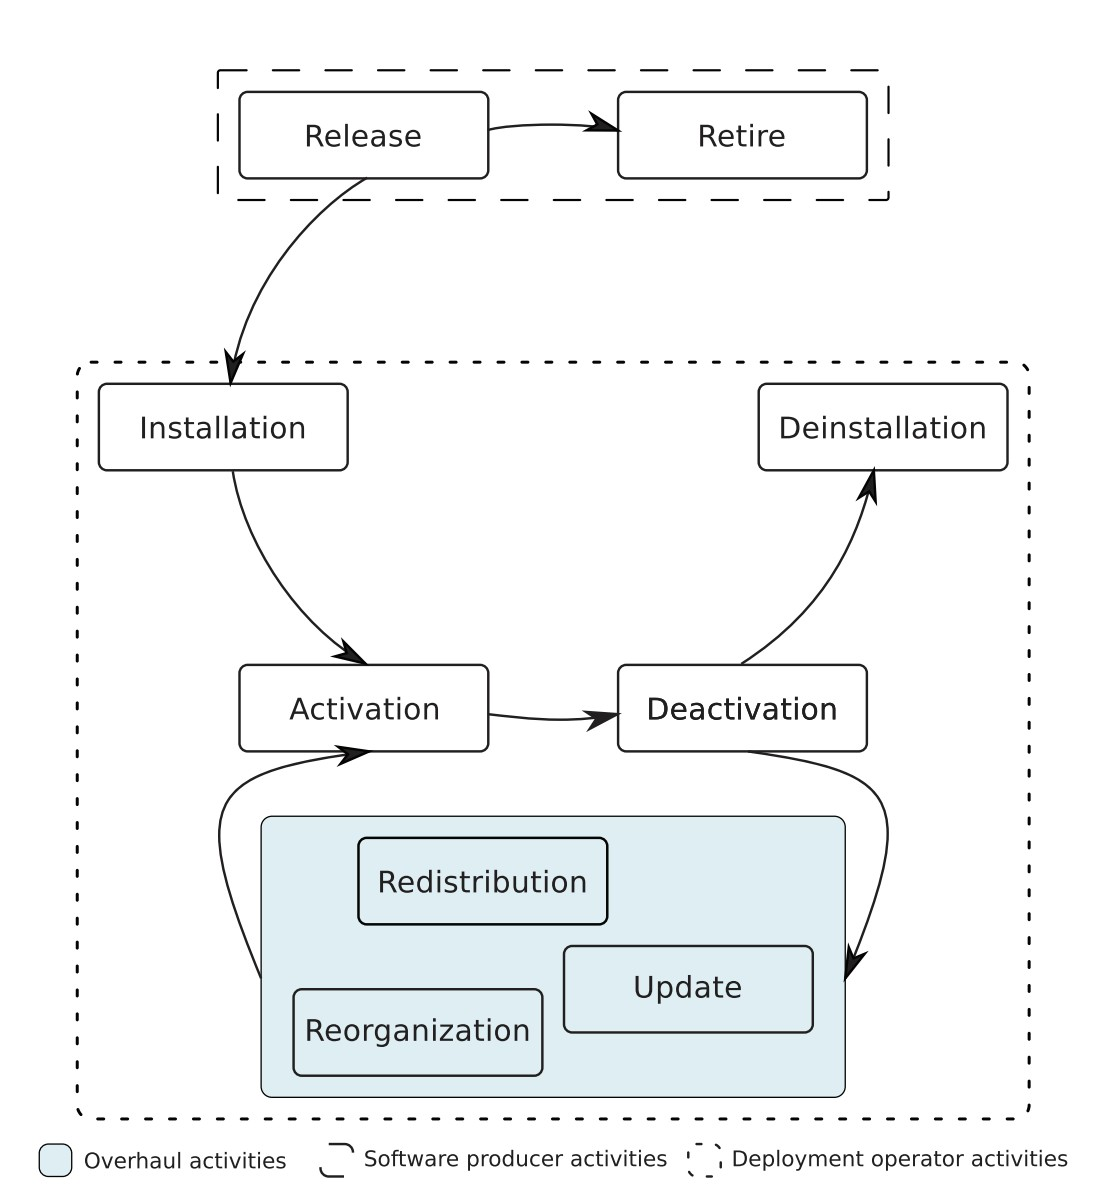
\includegraphics[width=0.8\textwidth]{resources/chapter-2/deployment-phase.jpg}
  \caption{\textit{Deployment Phase \parencite{ARCANGELI2015198}}}
  \label{fig:deployment-phase}
\end{figure}

\subsection{Sejarah}

Awal mulanya, \textit{deployment} dilakukan dengan membungkus \textit{software} menjadi sebuah \textit{installer}. \textit{Installer} dapat diunduh dan dijalankan oleh \textit{pengguna} untuk membuat \textit{software} tersedia pada perangkat yang digunakan. Jika terdapat \textit{update software}, pengguna harus mengunduh \textit{installer} dengan versi terbaru untuk digunakan \parencite{softwareDeploymentCarzaniga1998characterization}.

Hal ini tentunya kurang efektif karena pengguna harus melakukan pengecekan secara berkala untuk mengetahui apakah terdapat versi terbaru atau tidak. Oleh karena itu, muncul teknologi \textit{deployment} yaitu \textit{package manager}. \textit{Package Manager} dapat digunakan untuk proses \textit{installing, updating, and generally managing software} \parencite{softwareDeploymentCarzaniga1998characterization}. Namun, muncul beberapa masalah, seperti \textit{dependency hell}, \textit{dependency conflict}, serta \textit{platfrom-constrained} karena \textit{package manager} tidak tersedia di semua \textit{operating system}.

Pada tahun 2014, muncul teknologi baru yaitu \textit{docker, a cloud-centric platform-as-a-service} yang bertujuan untuk menyelesaikan masalah \textit{dependency conflict dan dependency hell} \parencite{merkel2014docker}. Docker menerapkan \textit{deployment} berbasis \textit{container} yang menggunakan namespace pada linux kernel dan cgroups dalam melakukan manajemen \textit{resource}-nya sehingga dapat membuat sistem berjalan secara khusus dengan seminimal mungkin tanpa konflik pada \textit{dependency}. Dengan adanya docker, mulai bermunculan banyak teknologi baru yang berfokus pada \textit{container} seperti \textit{podman dan kubernetes} serta \textit{deployment} mulai beralih pada \textit{cloud based deployment}.

\subsection{Kategori}
Pada penelitian yang dilakukan oleh \parencite{wurster2020essential}, \textit{deployment} dapat dikategorikan menjadi tiga bagian, yaitu \textit{General-Purpose (GP)}, \textit{Provider-Specific (ProvS)}, serta \textit{Platform-Specific (PlatS)}. Ketiga kategori ini berfokus untuk melakukan \textit{deployment} secara otomatis.

\begin{enumerate}
  \item \textit{General-Purpose} (GP)

        Teknologi ini mendukung semua fitur dan mekanisme \textit{deployment} mulai dari \textit{single-cloud}, \textit{hybrid}, \textit{multi-cloud}, serta berbagai jenis \textit{layanan cloud (XaaS)}. Beberapa teknologi yang ada pada kategori ini: Puppet, Chef, Ansible, OpenStack Heat, Terraform, SaltStack, Juju, dan Cloudify.

  \item \textit{Provider-Specific} (ProvS)

        Kategori ini menyediakan fitur untuk membuat \textit{reusable entity}. ProvS hanya mendukung \textit{deployment single-cloud} karena ditawarkan oleh penyedia \textit{cloud} tertentu, sehingga hanya mendukung layanan cloud yang ditawarkan oleh penyedia tersebut. Beberapa teknologi yang ada pada kategori ini: AWS CloudFormation dan Azure Resource Manager.

  \item \textit{Platform-Specific} (PlatS)

        Kategori ini mendukung \textit{multi-cloud} dan \textit{reusable deployment}. Kategori ini dibatasi dalam hal model pengiriman dan penggunaan bundel pada platform tertentu untuk membuat \textit{deployment}. Misalnya, Kubernetes hanya \textit{deployment} dengan \textit{container}. Beberapa teknologi yang ada pada kategori ini: Kubernetes, CFEngine, dan Docker Compose.

\end{enumerate}



